\documentclass[11pt]{article}
\usepackage[a4paper,top=0.6cm,bottom=3.0cm,left=1.9cm,right=1.9cm,footskip=2.0cm]{geometry}
\usepackage{graphicx}
\usepackage[table]{xcolor}
\usepackage{ragged2e}
\usepackage{fancyhdr}
\usepackage{fontspec}
\setmainfont{Noto Sans Telugu}
\setsansfont{Noto Sans Telugu}
\newfontfamily\latinfont{Carlito}
\renewcommand{\familydefault}{\sfdefault}
\definecolor{titleblue}{HTML}{0F2F4A}
\definecolor{textblack}{HTML}{1A1A1A}
\definecolor{rule}{HTML}{C9C4C0}
\definecolor{muted}{HTML}{6B635E}
\setlength{\parindent}{0pt}\setlength{\parskip}{0.5em}

\setlength{\headheight}{28pt}\setlength{\headsep}{6pt}
\newcommand{\idmfooter}{%
  \begin{minipage}{\textwidth}
    {\color{rule}\hrule height 0.7pt}\vspace{4pt}
    \noindent
    \begin{minipage}[c]{0.66\textwidth}{\scriptsize\color{muted}{\latinfont Developed by the Water and Climate Lab, IIT Gandhinagar, using hydro-meteorological data from partner agencies}.}\end{minipage}\hfill
    \begin{minipage}[c]{0.32\textwidth}\raggedleft
      
\includegraphics[height=0.62cm]{wcl.png}\hspace{6pt}%
      
\includegraphics[height=0.62cm]{iitgn.png}
    \end{minipage}\\[3pt]
    {\scriptsize\color{muted}© {\latinfont 2026 Water and Climate Lab} · {\latinfont Indian Institute of Technology Gandhinagar} · {\latinfont For research and demonstration purposes}.}
  \end{minipage}%
}
\newcommand{\idmrunhead}{%
  \begin{minipage}{\textwidth}
    {\small\bfseries\color{titleblue}{\latinfont National Drought Summary}}\hfill{\small\color{muted}{\latinfont Week ending May 20, 2026}}\\[2pt]
    {\color{rule}\hrule height 0.6pt}
  \end{minipage}%
}
\fancypagestyle{idmfoot}{\fancyhf{}\renewcommand{\headrulewidth}{0pt}\renewcommand{\footrulewidth}{0pt}\fancyfoot[C]{\idmfooter}}
\fancypagestyle{idmrun}{\fancyhf{}\renewcommand{\headrulewidth}{0pt}\renewcommand{\footrulewidth}{0pt}\fancyhead[C]{\idmrunhead}\fancyfoot[C]{\idmfooter}}
\pagestyle{idmrun}

\begin{document}

\thispagestyle{idmfoot}
\noindent
\begin{minipage}[c]{0.16\textwidth}
\includegraphics[width=\linewidth]{wcl.png}\end{minipage}\hfill
\begin{minipage}[c]{0.80\textwidth}\raggedleft
  {\fontsize{19}{22}\selectfont\bfseries\color{titleblue}{\latinfont National Drought Summary}}\\[2pt]
  {\normalsize\color{muted}{\latinfont Week ending May 20, 2026}}
\end{minipage}
\vspace{6pt}{\color{rule}\hrule height 1pt}\vspace{10pt}
\begin{center}
  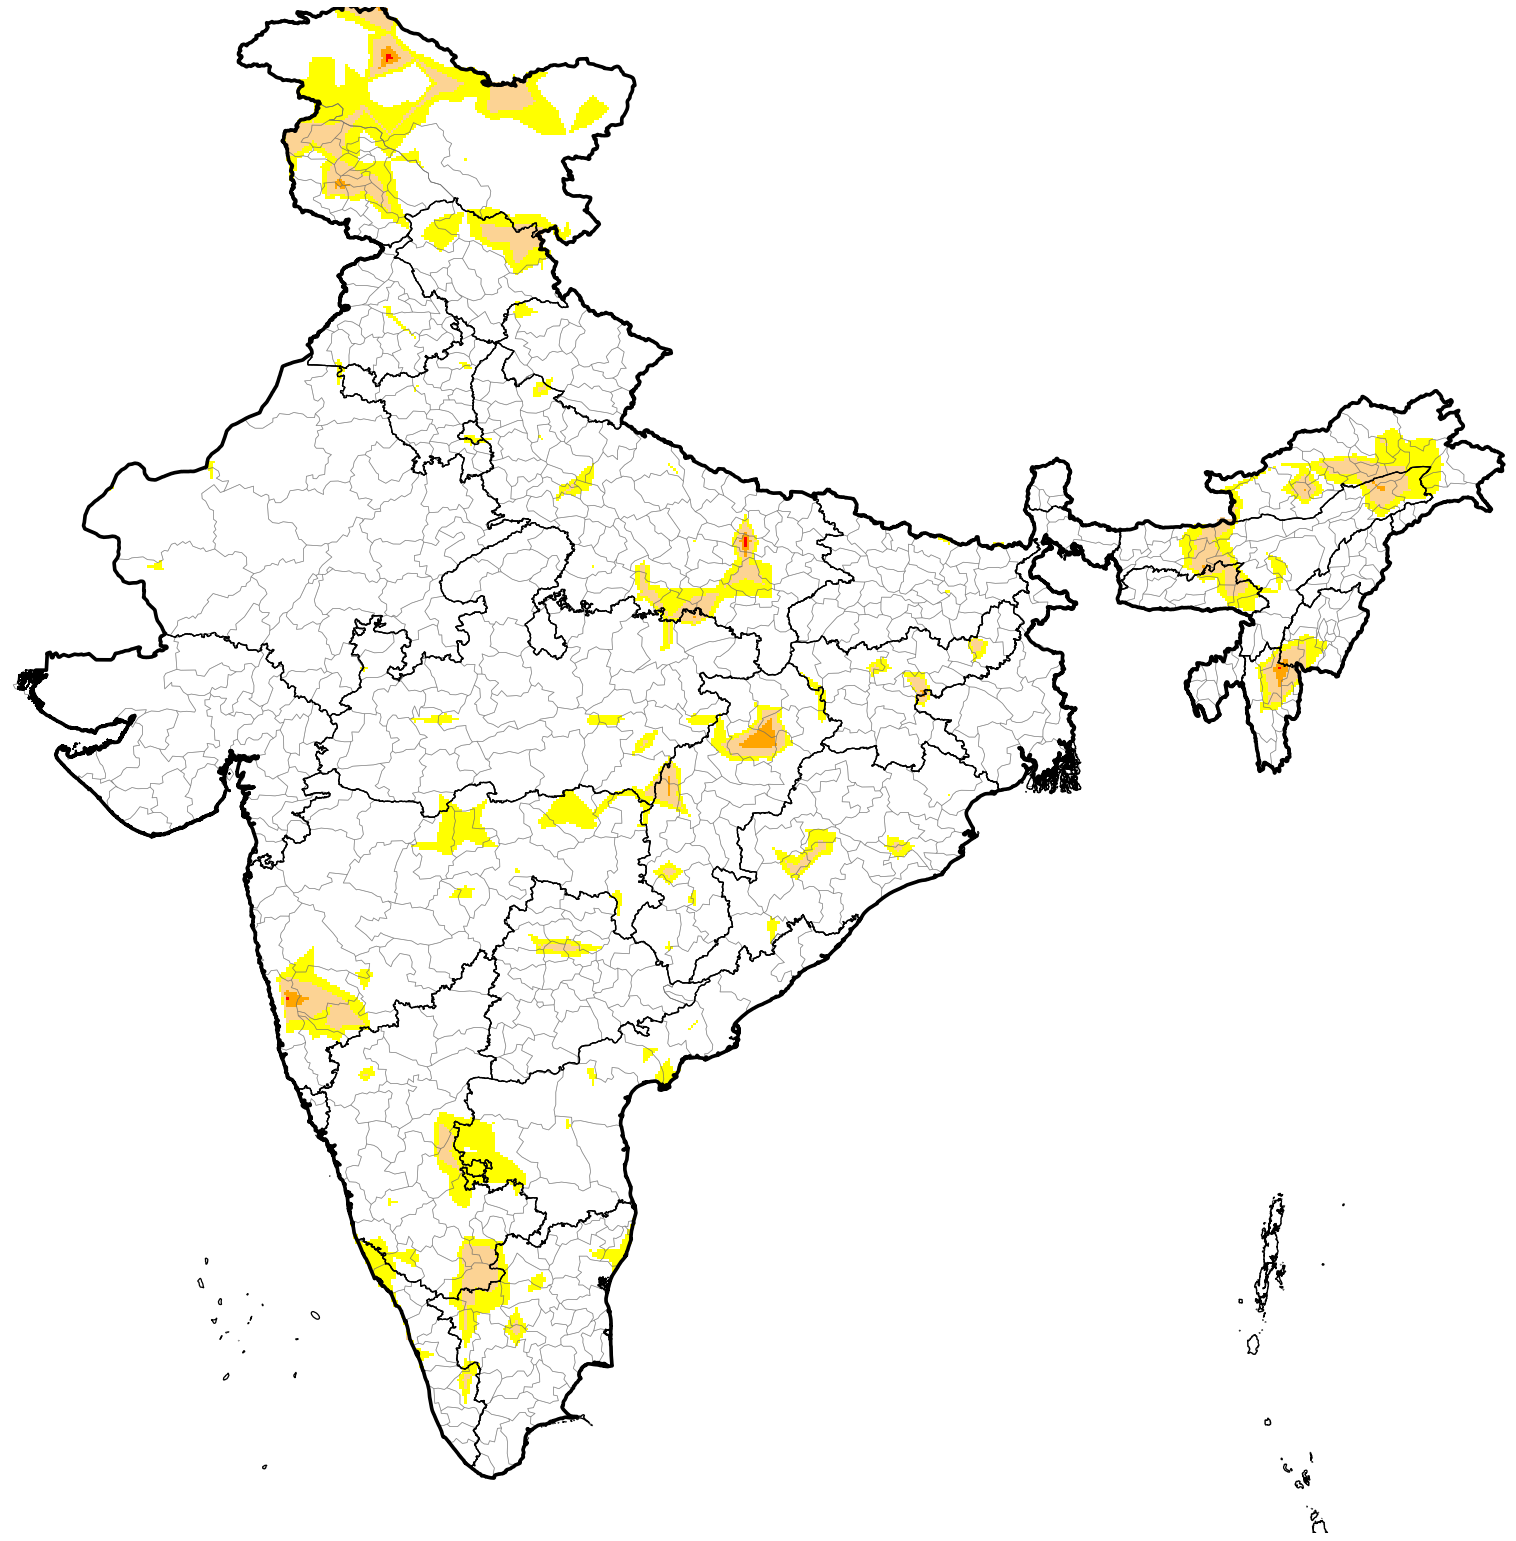
\includegraphics[width=0.60\textwidth]{cdi_map.png}\\[3pt]
  {\small\color{muted}{\latinfont Combined Drought Index (CDI) for the week ending May 20, 2026}.}
\end{center}
\vspace{2pt}
{\large\bfseries\color{titleblue}{\latinfont Summary}}\\[3pt]
{\justifying\normalsize\color{textblack}ఈ వారం జాతీయ కరువు పరిస్థితిలో ఎక్కువ ప్రాంతాలు సాధారణ వర్గంలో ఉన్నాయి, కొద్ది భాగం కరువు పరిస్థితులను అనుభవిస్తోంది. ఈ వారం భారతదేశంలో డి{\latinfont 0} లేదా అంతకంటే చెత్త వర్గంలో ఉన్న మొత్తం ప్రాంతం {\latinfont 15.3}\%గా ఉంది. ఇది గత వారం కంటే తగ్గుదల, వారంవారీగా మొత్తం కరువు ప్రాంతం {\latinfont 0.9} శాతం పాయింట్లు తగ్గింది. కరువు ప్రభావంలో ఎక్కువగా ఉన్న ప్రాంతాలు ఢిల్లీ {\latinfont NCT}, మణిపూర్, మిజోరామ్, అరుణాచల్ ప్రదేశ్, జమ్మూ కాశ్మీర్ మరియు మేఘాలయ. మరోవైపు, పశ్చిమ బెంగాల్ {\latinfont 0.0}\% ప్రాంతంలో కరువును నివేదించింది, రాజస్థాన్, గుజరాత్ మరియు తెలంగాణ వరుసగా {\latinfont 1.0}\%, {\latinfont 2.1}\% మరియు {\latinfont 3.4}\% ప్రాంతాలలో కరువును నివేదించాయి.\par}
\vspace{8pt}
{\large\bfseries\color{titleblue}{\latinfont Regional Outlook}}\\[2pt]
{\normalsize\color{titleblue}\textbf{{\latinfont North}}}\enspace {\normalsize\color{textblack}{\latinfont Moderate, scattered drought. About 28}\% {\latinfont of the area is in drought (D0}–{\latinfont D4)}.} \par\smallskip {\normalsize\color{titleblue}\textbf{{\latinfont Northwest}}}\enspace {\normalsize\color{textblack}{\latinfont Largely normal conditions. About 4}\% {\latinfont of the area is in drought (D0}–{\latinfont D4)}.} \par\smallskip {\normalsize\color{titleblue}\textbf{{\latinfont Northeast}}}\enspace {\normalsize\color{textblack}{\latinfont Moderate, scattered drought. About 27}\% {\latinfont of the area is in drought (D0}–{\latinfont D4). Pockets of severe-or-worse conditions are present}.} \par\smallskip {\normalsize\color{titleblue}\textbf{{\latinfont East}}}\enspace {\normalsize\color{textblack}{\latinfont Mostly normal, with localised dryness. About 7}\% {\latinfont of the area is in drought (D0}–{\latinfont D4)}.} \par\smallskip {\normalsize\color{titleblue}\textbf{{\latinfont Central}}}\enspace {\normalsize\color{textblack}{\latinfont Mostly normal, with localised dryness. About 15}\% {\latinfont of the area is in drought (D0}–{\latinfont D4). Pockets of severe-or-worse conditions are present}.} \par\smallskip {\normalsize\color{titleblue}\textbf{{\latinfont West}}}\enspace {\normalsize\color{textblack}{\latinfont Moderate, scattered drought. About 22}\% {\latinfont of the area is in drought (D0}–{\latinfont D4)}.} \par\smallskip {\normalsize\color{titleblue}\textbf{{\latinfont South}}}\enspace {\normalsize\color{textblack}{\latinfont Mostly normal, with localised dryness. About 16}\% {\latinfont of the area is in drought (D0}–{\latinfont D4)}.}
\end{document}
